% Created by tikzDevice version 0.8.1 on 2015-11-15 17:38:49
% !TEX encoding = UTF-8 Unicode
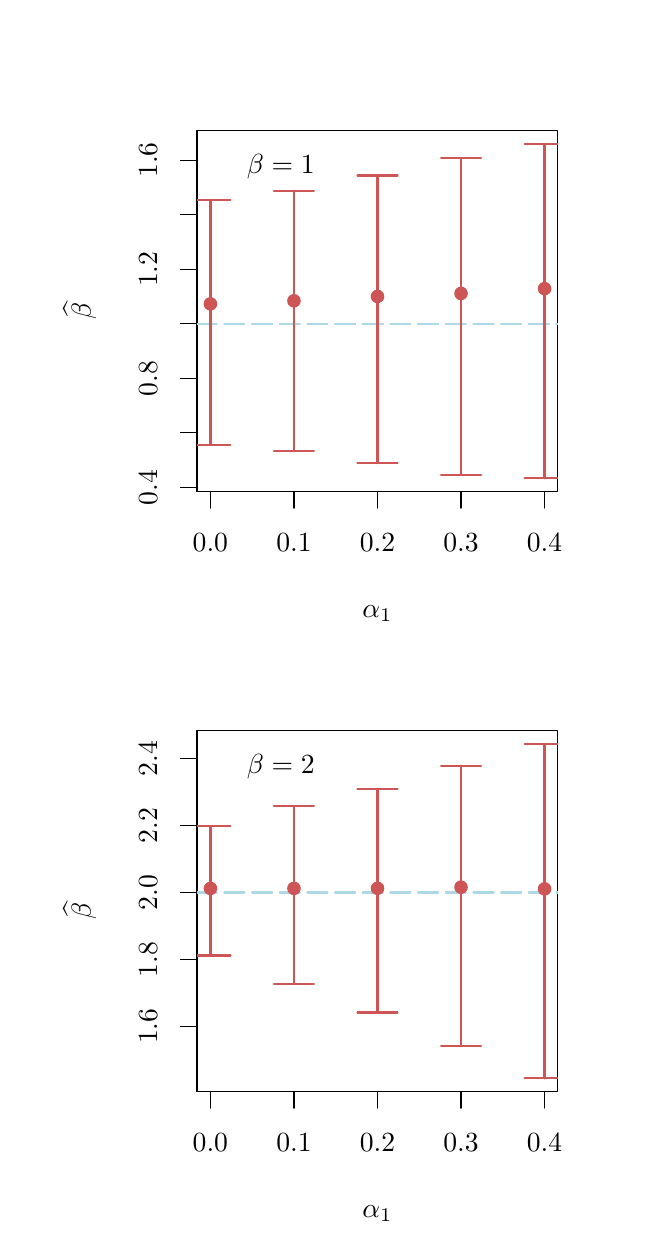
\begin{tikzpicture}[x=1pt,y=1pt]
\definecolor{fillColor}{RGB}{255,255,255}
\path[use as bounding box,fill=fillColor,fill opacity=0.00] (0,0) rectangle (216.81,433.62);
\begin{scope}
\path[clip] ( 61.20,266.01) rectangle (191.61,396.42);
\definecolor{drawColor}{RGB}{255,255,255}
\definecolor{fillColor}{RGB}{255,255,255}

\path[draw=drawColor,line width= 0.4pt,line join=round,line cap=round,fill=fillColor] ( 66.03,333.81) circle (  2.25);

\path[draw=drawColor,line width= 0.4pt,line join=round,line cap=round,fill=fillColor] ( 96.22,334.92) circle (  2.25);

\path[draw=drawColor,line width= 0.4pt,line join=round,line cap=round,fill=fillColor] (126.41,336.50) circle (  2.25);

\path[draw=drawColor,line width= 0.4pt,line join=round,line cap=round,fill=fillColor] (156.59,337.58) circle (  2.25);

\path[draw=drawColor,line width= 0.4pt,line join=round,line cap=round,fill=fillColor] (186.78,339.31) circle (  2.25);
\end{scope}
\begin{scope}
\path[clip] (  0.00,  0.00) rectangle (216.81,433.62);
\definecolor{drawColor}{RGB}{0,0,0}

\path[draw=drawColor,line width= 0.4pt,line join=round,line cap=round] ( 66.03,266.01) -- (186.78,266.01);

\path[draw=drawColor,line width= 0.4pt,line join=round,line cap=round] ( 66.03,266.01) -- ( 66.03,260.01);

\path[draw=drawColor,line width= 0.4pt,line join=round,line cap=round] ( 96.22,266.01) -- ( 96.22,260.01);

\path[draw=drawColor,line width= 0.4pt,line join=round,line cap=round] (126.41,266.01) -- (126.41,260.01);

\path[draw=drawColor,line width= 0.4pt,line join=round,line cap=round] (156.59,266.01) -- (156.59,260.01);

\path[draw=drawColor,line width= 0.4pt,line join=round,line cap=round] (186.78,266.01) -- (186.78,260.01);

\node[text=drawColor,anchor=base,inner sep=0pt, outer sep=0pt, scale=  1.00] at ( 66.03,244.41) {0.0};

\node[text=drawColor,anchor=base,inner sep=0pt, outer sep=0pt, scale=  1.00] at ( 96.22,244.41) {0.1};

\node[text=drawColor,anchor=base,inner sep=0pt, outer sep=0pt, scale=  1.00] at (126.41,244.41) {0.2};

\node[text=drawColor,anchor=base,inner sep=0pt, outer sep=0pt, scale=  1.00] at (156.59,244.41) {0.3};

\node[text=drawColor,anchor=base,inner sep=0pt, outer sep=0pt, scale=  1.00] at (186.78,244.41) {0.4};

\path[draw=drawColor,line width= 0.4pt,line join=round,line cap=round] ( 61.20,267.47) -- ( 61.20,385.77);

\path[draw=drawColor,line width= 0.4pt,line join=round,line cap=round] ( 61.20,267.47) -- ( 55.20,267.47);

\path[draw=drawColor,line width= 0.4pt,line join=round,line cap=round] ( 61.20,287.18) -- ( 55.20,287.18);

\path[draw=drawColor,line width= 0.4pt,line join=round,line cap=round] ( 61.20,306.90) -- ( 55.20,306.90);

\path[draw=drawColor,line width= 0.4pt,line join=round,line cap=round] ( 61.20,326.62) -- ( 55.20,326.62);

\path[draw=drawColor,line width= 0.4pt,line join=round,line cap=round] ( 61.20,346.33) -- ( 55.20,346.33);

\path[draw=drawColor,line width= 0.4pt,line join=round,line cap=round] ( 61.20,366.05) -- ( 55.20,366.05);

\path[draw=drawColor,line width= 0.4pt,line join=round,line cap=round] ( 61.20,385.77) -- ( 55.20,385.77);

\node[text=drawColor,rotate= 90.00,anchor=base,inner sep=0pt, outer sep=0pt, scale=  1.00] at ( 46.80,267.47) {0.4};

\node[text=drawColor,rotate= 90.00,anchor=base,inner sep=0pt, outer sep=0pt, scale=  1.00] at ( 46.80,306.90) {0.8};

\node[text=drawColor,rotate= 90.00,anchor=base,inner sep=0pt, outer sep=0pt, scale=  1.00] at ( 46.80,346.33) {1.2};

\node[text=drawColor,rotate= 90.00,anchor=base,inner sep=0pt, outer sep=0pt, scale=  1.00] at ( 46.80,385.77) {1.6};

\path[draw=drawColor,line width= 0.4pt,line join=round,line cap=round] ( 61.20,266.01) --
	(191.61,266.01) --
	(191.61,396.42) --
	( 61.20,396.42) --
	( 61.20,266.01);
\end{scope}
\begin{scope}
\path[clip] (  0.00,216.81) rectangle (216.81,433.62);
\definecolor{drawColor}{RGB}{0,0,0}

\node[text=drawColor,anchor=base,inner sep=0pt, outer sep=0pt, scale=  1.00] at (126.41,220.41) {$\alpha_1$};

\node[text=drawColor,rotate= 90.00,anchor=base,inner sep=0pt, outer sep=0pt, scale=  1.00] at ( 22.80,331.22) {$\widehat{\beta}$};
\end{scope}
\begin{scope}
\path[clip] ( 61.20,266.01) rectangle (191.61,396.42);
\definecolor{drawColor}{RGB}{0,0,0}

\node[text=drawColor,anchor=base west,inner sep=0pt, outer sep=0pt, scale=  1.00] at ( 79.20,380.98) {$\beta=1$};
\definecolor{drawColor}{RGB}{173,216,230}

\path[draw=drawColor,line width= 0.8pt,dash pattern=on 7pt off 3pt ,line join=round,line cap=round] ( 61.20,326.62) -- (191.61,326.62);

\path[draw=drawColor,line width= 0.8pt,dash pattern=on 7pt off 3pt ,line join=round,line cap=round] ( 61.20,326.62) -- (191.61,326.62);

\path[draw=drawColor,line width= 0.8pt,dash pattern=on 7pt off 3pt ,line join=round,line cap=round] ( 61.20,326.62) -- (191.61,326.62);

\path[draw=drawColor,line width= 0.8pt,dash pattern=on 7pt off 3pt ,line join=round,line cap=round] ( 61.20,326.62) -- (191.61,326.62);

\path[draw=drawColor,line width= 0.8pt,dash pattern=on 7pt off 3pt ,line join=round,line cap=round] ( 61.20,326.62) -- (191.61,326.62);
\definecolor{drawColor}{RGB}{205,85,85}

\path[draw=drawColor,line width= 0.8pt,line join=round,line cap=round] ( 66.03,282.88) -- ( 66.03,371.32);

\path[draw=drawColor,line width= 0.8pt,line join=round,line cap=round] ( 58.80,282.88) --
	( 66.03,282.88) --
	( 73.26,282.88);

\path[draw=drawColor,line width= 0.8pt,line join=round,line cap=round] ( 73.26,371.32) --
	( 66.03,371.32) --
	( 58.80,371.32);

\path[draw=drawColor,line width= 0.8pt,line join=round,line cap=round] ( 96.22,280.61) -- ( 96.22,374.69);

\path[draw=drawColor,line width= 0.8pt,line join=round,line cap=round] ( 88.99,280.61) --
	( 96.22,280.61) --
	(103.44,280.61);

\path[draw=drawColor,line width= 0.8pt,line join=round,line cap=round] (103.44,374.69) --
	( 96.22,374.69) --
	( 88.99,374.69);

\path[draw=drawColor,line width= 0.8pt,line join=round,line cap=round] (126.41,276.27) -- (126.41,380.23);

\path[draw=drawColor,line width= 0.8pt,line join=round,line cap=round] (119.18,276.27) --
	(126.41,276.27) --
	(133.63,276.27);

\path[draw=drawColor,line width= 0.8pt,line join=round,line cap=round] (133.63,380.23) --
	(126.41,380.23) --
	(119.18,380.23);

\path[draw=drawColor,line width= 0.8pt,line join=round,line cap=round] (156.59,272.02) -- (156.59,386.58);

\path[draw=drawColor,line width= 0.8pt,line join=round,line cap=round] (149.37,272.02) --
	(156.59,272.02) --
	(163.82,272.02);

\path[draw=drawColor,line width= 0.8pt,line join=round,line cap=round] (163.82,386.58) --
	(156.59,386.58) --
	(149.37,386.58);

\path[draw=drawColor,line width= 0.8pt,line join=round,line cap=round] (186.78,270.84) -- (186.78,391.59);

\path[draw=drawColor,line width= 0.8pt,line join=round,line cap=round] (179.55,270.84) --
	(186.78,270.84) --
	(194.01,270.84);

\path[draw=drawColor,line width= 0.8pt,line join=round,line cap=round] (194.01,391.59) --
	(186.78,391.59) --
	(179.55,391.59);
\definecolor{fillColor}{RGB}{205,85,85}

\path[draw=drawColor,line width= 0.4pt,line join=round,line cap=round,fill=fillColor] ( 66.03,333.81) circle (  2.25);

\path[draw=drawColor,line width= 0.4pt,line join=round,line cap=round,fill=fillColor] ( 96.22,334.92) circle (  2.25);

\path[draw=drawColor,line width= 0.4pt,line join=round,line cap=round,fill=fillColor] (126.41,336.50) circle (  2.25);

\path[draw=drawColor,line width= 0.4pt,line join=round,line cap=round,fill=fillColor] (156.59,337.58) circle (  2.25);

\path[draw=drawColor,line width= 0.4pt,line join=round,line cap=round,fill=fillColor] (186.78,339.31) circle (  2.25);
\end{scope}
\begin{scope}
\path[clip] ( 61.20, 49.20) rectangle (191.61,179.61);
\definecolor{drawColor}{RGB}{255,255,255}
\definecolor{fillColor}{RGB}{255,255,255}

\path[draw=drawColor,line width= 0.4pt,line join=round,line cap=round,fill=fillColor] ( 66.03,122.58) circle (  2.25);

\path[draw=drawColor,line width= 0.4pt,line join=round,line cap=round,fill=fillColor] ( 96.22,122.61) circle (  2.25);

\path[draw=drawColor,line width= 0.4pt,line join=round,line cap=round,fill=fillColor] (126.41,122.64) circle (  2.25);

\path[draw=drawColor,line width= 0.4pt,line join=round,line cap=round,fill=fillColor] (156.59,123.04) circle (  2.25);

\path[draw=drawColor,line width= 0.4pt,line join=round,line cap=round,fill=fillColor] (186.78,122.42) circle (  2.25);
\end{scope}
\begin{scope}
\path[clip] (  0.00,  0.00) rectangle (216.81,433.62);
\definecolor{drawColor}{RGB}{0,0,0}

\path[draw=drawColor,line width= 0.4pt,line join=round,line cap=round] ( 66.03, 49.20) -- (186.78, 49.20);

\path[draw=drawColor,line width= 0.4pt,line join=round,line cap=round] ( 66.03, 49.20) -- ( 66.03, 43.20);

\path[draw=drawColor,line width= 0.4pt,line join=round,line cap=round] ( 96.22, 49.20) -- ( 96.22, 43.20);

\path[draw=drawColor,line width= 0.4pt,line join=round,line cap=round] (126.41, 49.20) -- (126.41, 43.20);

\path[draw=drawColor,line width= 0.4pt,line join=round,line cap=round] (156.59, 49.20) -- (156.59, 43.20);

\path[draw=drawColor,line width= 0.4pt,line join=round,line cap=round] (186.78, 49.20) -- (186.78, 43.20);

\node[text=drawColor,anchor=base,inner sep=0pt, outer sep=0pt, scale=  1.00] at ( 66.03, 27.60) {0.0};

\node[text=drawColor,anchor=base,inner sep=0pt, outer sep=0pt, scale=  1.00] at ( 96.22, 27.60) {0.1};

\node[text=drawColor,anchor=base,inner sep=0pt, outer sep=0pt, scale=  1.00] at (126.41, 27.60) {0.2};

\node[text=drawColor,anchor=base,inner sep=0pt, outer sep=0pt, scale=  1.00] at (156.59, 27.60) {0.3};

\node[text=drawColor,anchor=base,inner sep=0pt, outer sep=0pt, scale=  1.00] at (186.78, 27.60) {0.4};

\path[draw=drawColor,line width= 0.4pt,line join=round,line cap=round] ( 61.20, 72.78) -- ( 61.20,169.44);

\path[draw=drawColor,line width= 0.4pt,line join=round,line cap=round] ( 61.20, 72.78) -- ( 55.20, 72.78);

\path[draw=drawColor,line width= 0.4pt,line join=round,line cap=round] ( 61.20, 96.95) -- ( 55.20, 96.95);

\path[draw=drawColor,line width= 0.4pt,line join=round,line cap=round] ( 61.20,121.11) -- ( 55.20,121.11);

\path[draw=drawColor,line width= 0.4pt,line join=round,line cap=round] ( 61.20,145.28) -- ( 55.20,145.28);

\path[draw=drawColor,line width= 0.4pt,line join=round,line cap=round] ( 61.20,169.44) -- ( 55.20,169.44);

\node[text=drawColor,rotate= 90.00,anchor=base,inner sep=0pt, outer sep=0pt, scale=  1.00] at ( 46.80, 72.78) {1.6};

\node[text=drawColor,rotate= 90.00,anchor=base,inner sep=0pt, outer sep=0pt, scale=  1.00] at ( 46.80, 96.95) {1.8};

\node[text=drawColor,rotate= 90.00,anchor=base,inner sep=0pt, outer sep=0pt, scale=  1.00] at ( 46.80,121.11) {2.0};

\node[text=drawColor,rotate= 90.00,anchor=base,inner sep=0pt, outer sep=0pt, scale=  1.00] at ( 46.80,145.28) {2.2};

\node[text=drawColor,rotate= 90.00,anchor=base,inner sep=0pt, outer sep=0pt, scale=  1.00] at ( 46.80,169.44) {2.4};

\path[draw=drawColor,line width= 0.4pt,line join=round,line cap=round] ( 61.20, 49.20) --
	(191.61, 49.20) --
	(191.61,179.61) --
	( 61.20,179.61) --
	( 61.20, 49.20);
\end{scope}
\begin{scope}
\path[clip] (  0.00,  0.00) rectangle (216.81,216.81);
\definecolor{drawColor}{RGB}{0,0,0}

\node[text=drawColor,anchor=base,inner sep=0pt, outer sep=0pt, scale=  1.00] at (126.41,  3.60) {$\alpha_1$};

\node[text=drawColor,rotate= 90.00,anchor=base,inner sep=0pt, outer sep=0pt, scale=  1.00] at ( 22.80,114.41) {$\widehat{\beta}$};
\end{scope}
\begin{scope}
\path[clip] ( 61.20, 49.20) rectangle (191.61,179.61);
\definecolor{drawColor}{RGB}{0,0,0}

\node[text=drawColor,anchor=base west,inner sep=0pt, outer sep=0pt, scale=  1.00] at ( 79.20,164.17) {$\beta=2$};
\definecolor{drawColor}{RGB}{173,216,230}

\path[draw=drawColor,line width= 0.8pt,dash pattern=on 7pt off 3pt ,line join=round,line cap=round] ( 61.20,121.11) -- (191.61,121.11);

\path[draw=drawColor,line width= 0.8pt,dash pattern=on 7pt off 3pt ,line join=round,line cap=round] ( 61.20,121.11) -- (191.61,121.11);

\path[draw=drawColor,line width= 0.8pt,dash pattern=on 7pt off 3pt ,line join=round,line cap=round] ( 61.20,121.11) -- (191.61,121.11);

\path[draw=drawColor,line width= 0.8pt,dash pattern=on 7pt off 3pt ,line join=round,line cap=round] ( 61.20,121.11) -- (191.61,121.11);

\path[draw=drawColor,line width= 0.8pt,dash pattern=on 7pt off 3pt ,line join=round,line cap=round] ( 61.20,121.11) -- (191.61,121.11);
\definecolor{drawColor}{RGB}{205,85,85}

\path[draw=drawColor,line width= 0.8pt,line join=round,line cap=round] ( 66.03, 98.36) -- ( 66.03,145.04);

\path[draw=drawColor,line width= 0.8pt,line join=round,line cap=round] ( 58.80, 98.36) --
	( 66.03, 98.36) --
	( 73.26, 98.36);

\path[draw=drawColor,line width= 0.8pt,line join=round,line cap=round] ( 73.26,145.04) --
	( 66.03,145.04) --
	( 58.80,145.04);

\path[draw=drawColor,line width= 0.8pt,line join=round,line cap=round] ( 96.22, 88.09) -- ( 96.22,152.33);

\path[draw=drawColor,line width= 0.8pt,line join=round,line cap=round] ( 88.99, 88.09) --
	( 96.22, 88.09) --
	(103.44, 88.09);

\path[draw=drawColor,line width= 0.8pt,line join=round,line cap=round] (103.44,152.33) --
	( 96.22,152.33) --
	( 88.99,152.33);

\path[draw=drawColor,line width= 0.8pt,line join=round,line cap=round] (126.41, 77.76) -- (126.41,158.49);

\path[draw=drawColor,line width= 0.8pt,line join=round,line cap=round] (119.18, 77.76) --
	(126.41, 77.76) --
	(133.63, 77.76);

\path[draw=drawColor,line width= 0.8pt,line join=round,line cap=round] (133.63,158.49) --
	(126.41,158.49) --
	(119.18,158.49);

\path[draw=drawColor,line width= 0.8pt,line join=round,line cap=round] (156.59, 65.74) -- (156.59,166.94);

\path[draw=drawColor,line width= 0.8pt,line join=round,line cap=round] (149.37, 65.74) --
	(156.59, 65.74) --
	(163.82, 65.74);

\path[draw=drawColor,line width= 0.8pt,line join=round,line cap=round] (163.82,166.94) --
	(156.59,166.94) --
	(149.37,166.94);

\path[draw=drawColor,line width= 0.8pt,line join=round,line cap=round] (186.78, 54.03) -- (186.78,174.78);

\path[draw=drawColor,line width= 0.8pt,line join=round,line cap=round] (179.55, 54.03) --
	(186.78, 54.03) --
	(194.01, 54.03);

\path[draw=drawColor,line width= 0.8pt,line join=round,line cap=round] (194.01,174.78) --
	(186.78,174.78) --
	(179.55,174.78);
\definecolor{fillColor}{RGB}{205,85,85}

\path[draw=drawColor,line width= 0.4pt,line join=round,line cap=round,fill=fillColor] ( 66.03,122.58) circle (  2.25);

\path[draw=drawColor,line width= 0.4pt,line join=round,line cap=round,fill=fillColor] ( 96.22,122.61) circle (  2.25);

\path[draw=drawColor,line width= 0.4pt,line join=round,line cap=round,fill=fillColor] (126.41,122.64) circle (  2.25);

\path[draw=drawColor,line width= 0.4pt,line join=round,line cap=round,fill=fillColor] (156.59,123.04) circle (  2.25);

\path[draw=drawColor,line width= 0.4pt,line join=round,line cap=round,fill=fillColor] (186.78,122.42) circle (  2.25);
\end{scope}
\end{tikzpicture}
